\documentclass[a4paper]{article}

\usepackage[utf8]{inputenc}
\usepackage[portuguese]{babel}
\usepackage{graphicx}
\graphicspath{ {Imagens/} }

\title{Trabalho Prático 1 de Processamento de Linguagens}
\author{André Vieira (A78322) \and Eduardo Rocha (A77048) \and Ricardo Neves (A78764)}
\date{\today}

\begin{document}

\maketitle

\begin{abstract}
  Este documento apresenta o relatório do primeiro projeto de 
  Proessamento de Linguagens, da Licenciatura em Engenharia Informática da 
  Universidade do Minho.
\end{abstract}

\tableofcontents

\section{Introdução}
\label{sec:intro}

Este trabalho prático foi realizado no ambito da Unidade Curricular de Processamento de Linguagens.
Aqui, iremos dicutir toda a estratégia e linha de pensamento que o grupo tomou, de modo a cumprir os requisitos pedidos.

Uma vez que o menor número mecanográfico é igual a 77048, e ao dividir este mesmo número por 5, constatamos que o resto desta operação é igual a 3, que corresponde ao algarismo do enunciado pertencente.
Deste modo, o grupo constatou que o enunciado atribuido foi o 2.3 - Processador / sincronizador de legendas.
Este trabalho engloba, em geral, 2 exercícios distintos, que iremos mencionar mais à frente, em pormenor.
O objetivo máximo do grupo em relação a este trabalho foi o de realizar os dois exercicios pedidos com a maior eficiência, ganhando, assim, experiência e conhecimento em relação à ferramenta AWK, que irá ser importante no seguimento desta Unidade Curricular. Esta ferramenta permite manipular o texto de ficheiros, pesquisar e obter apenas certas palavras que estão contidas no mesmo, entre várias outas funcionalidades. Assim, este trabalho baseou-se na exploração destas mesmas funcionalidades que o AWK nos oferece.
Com o fecho da introdução deste relatório, é adequado mencionar a estrutura do mesmo. Este relatório contém o resumo do trabalho que foi realizado durante o período dado para tal, a descrição e a implementação dos dois exercícios que compõem o trabalho prático (incluíndo a linha de pensamento seguida pelo grupo, bem como imagens que ajudam à interpretação), e no final, uma pequena conclusão que reflete o trabalho realizado.


\section{Resumo}
\label{sec:resumo}

Este trabalho prático resume-se, então, à manipulação de legendas de filmes. 
Todas as legendas disponibilizadas seguem o seguinte formato:

\begin{center}
	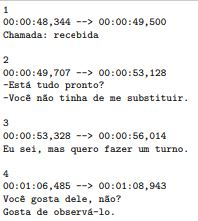
\includegraphics{1}
	\begin{figure}[!h]
	\caption{Exemplo de formato de legendas}
	\end{figure}
\end{center}

Como se pode observar na imagem acima, cada legenda apresenta o número que a caracteriza.
Na linha abaixo, podemos ver também o tempo de início e de fim da legenda. Ou seja, o tempo onde a mesma aparece e desaparece durante o percurso do filme. Se quisermos obter o tempo que a legenda manteu-se visível ao espectador, é necessário fazer a subtração entre o segundo número e o primeiro.
Por fim, vemos o corpo da legenda, isto é, o texto que fica visível ao utilizador.

Este template repete-se para todas as legendas diponíveis, o que facilitou o trabalho do grupo de certo modo, o que permite percorrer todas elas de uma forma semelhante.

\vspace{75px}
\section{Exercício 1}
\label{sec:ex1}

Este primeiro de dois exercícios desafiou o grupo de trabalho a transformar o modo como as legendas aparecem no ficheiro original.

Assim, o grupo construiu um processador que retira os identificadores das legendas, ou seja, a primeira linha de cada uma, coloque as legendas numa única linha, juntando-as com o caracter '$|$', e marcar com os caracteres '=' todos os intervalos de tempo com mais de 2 segundos de silencio.

Deste modo, foi contruída esta ferramenta.

\begin{center}
	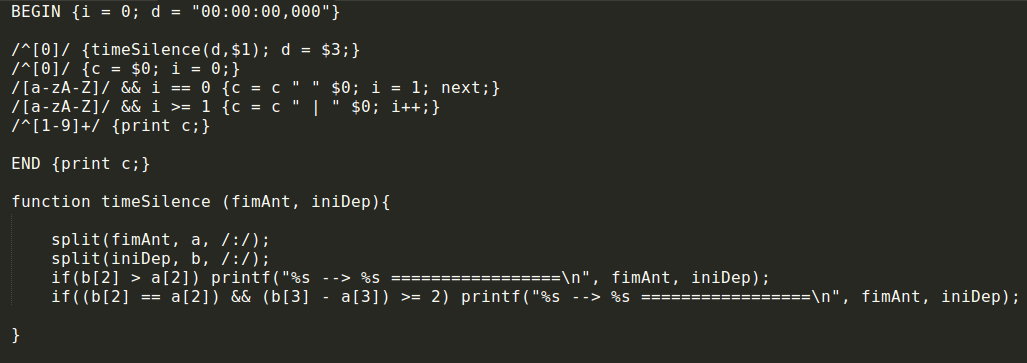
\includegraphics[scale=0.3]{2}
	\begin{figure}[!h]
	\caption{Código construído para exercício 1}
	\end{figure}
\end{center}

Ao observar atentamente o ficheiro das legendas original, constatamos que todos os tempos começavam com o algarismo 0. Deste modo, de modo a não imprimir o número que caracteriza a legenda, implementamos que, se a linha começar por 0, irá ser imprimida. No entanto, é aplicada a função auxiliar timeSilence, que irá ser explicada mais tarde.
De seguida, é necessário imprimir o texto da legenda. Assim, se a legenda contiver uma letra, também será imprimida. No entanto, se de seguida, for encontrada outra legenda (a sua segunda parte), irá ser imprimido o caracter '|', e só depois a segunda linha da mesma.

Falando um pouco acerca da função auxiliar timeSilence, este é o método que nos permite avaliar se existe alguem tempo de silêncio com uma duração maior do que 2 segundos.
Assim, esta função receve dois argumentos: o tempo final da primeira legenda, e o tempo inicial da segunda legenda. Como já foi mencionado, é aqui que estes tempos são subtraídos. Se este resultado for maior do que 2, uma série de caracteres '=' irão ser imprimidos, o que quer dizer que houve um tempo de silencio durante esta parte do filme. Se isto não se constatar, então o programa não imprimirá nada.

\vspace{200px}

Esta imagem representa as legendas no ficheiro original do filme Harry Potter:

\begin{center}
	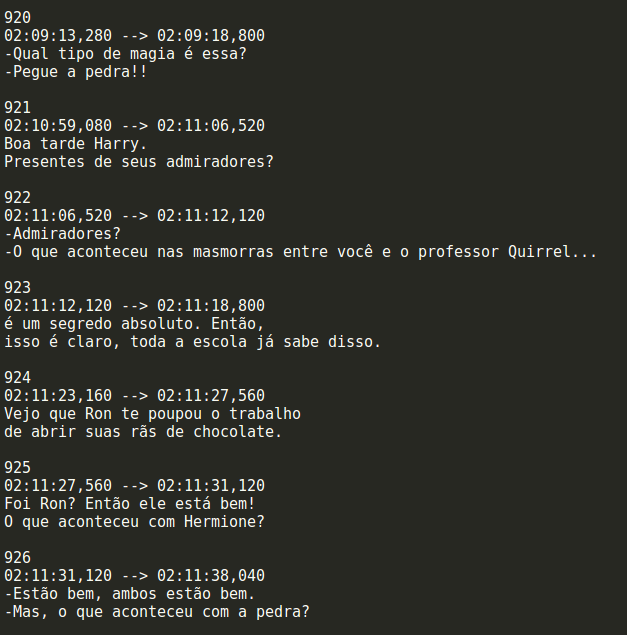
\includegraphics[scale=0.4]{3}
	\begin{figure}[!h]
	\caption{Legendas originais do filme Harry Potter}
	\end{figure}
\end{center}

Com a função implementada, corremos este comando AWK no terminal:

\begin{center}
	
\includegraphics[scale=0.7]{4}
	\begin{figure}[!h]
	\caption{Comando gawk utilizado}
	\end{figure}
\end{center}


\vspace{400px}
De imediato, recebemos o resultado final da transformação que foi executada:

\begin{center}
	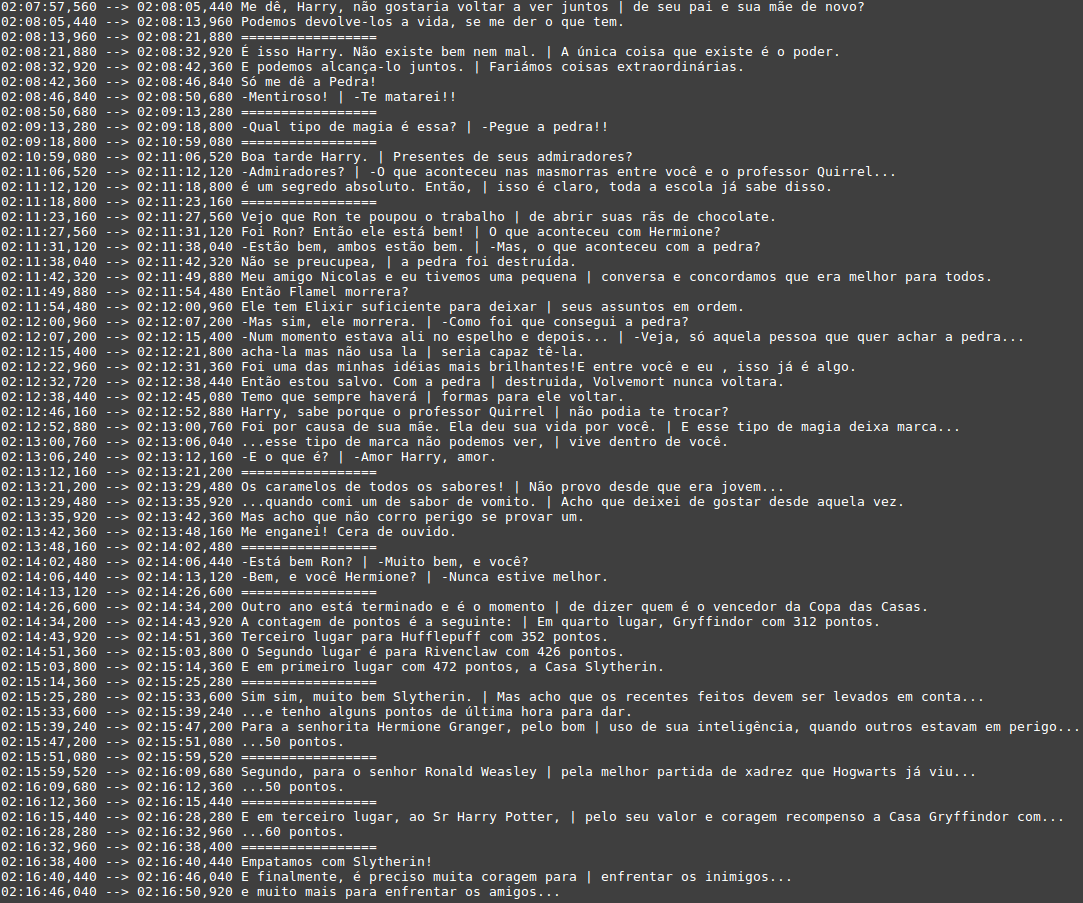
\includegraphics[scale=0.35]{5}
	\begin{figure}[!h]
	\caption{Legendas do filme Harry Potter modificadas}
	\end{figure}
\end{center}

\vspace{200px}
Para ter a certeza que tudo estava a funcionar corretamente, testamos o mesmo procedimento nas legendas do filme Ted:

\begin{center}
	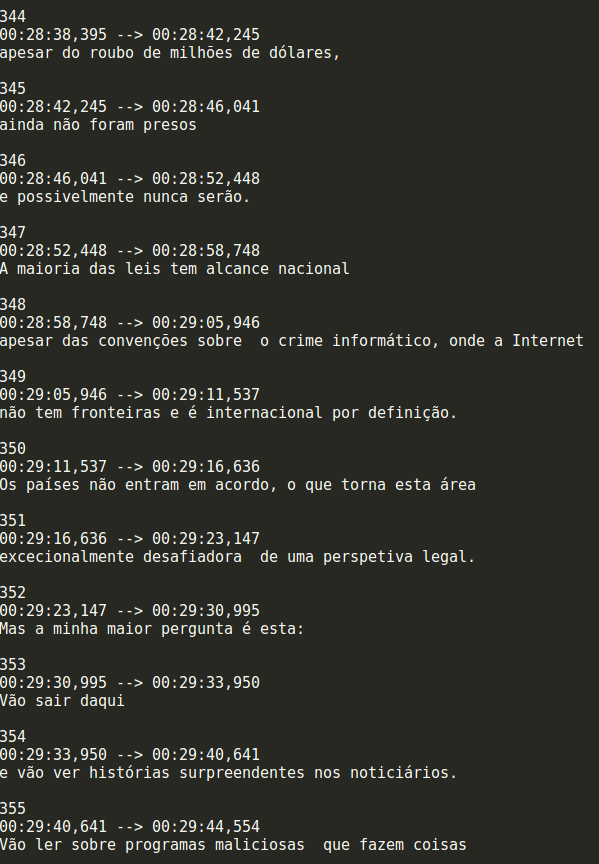
\includegraphics[scale=0.45]{6}
	\begin{figure}[!h]
	\caption{Legendas originais do filme Ted}
	\end{figure}
\end{center}

\vspace{200px}
Correndo o comando gawk, é devolvido o seguinte resultado:

\begin{center}
	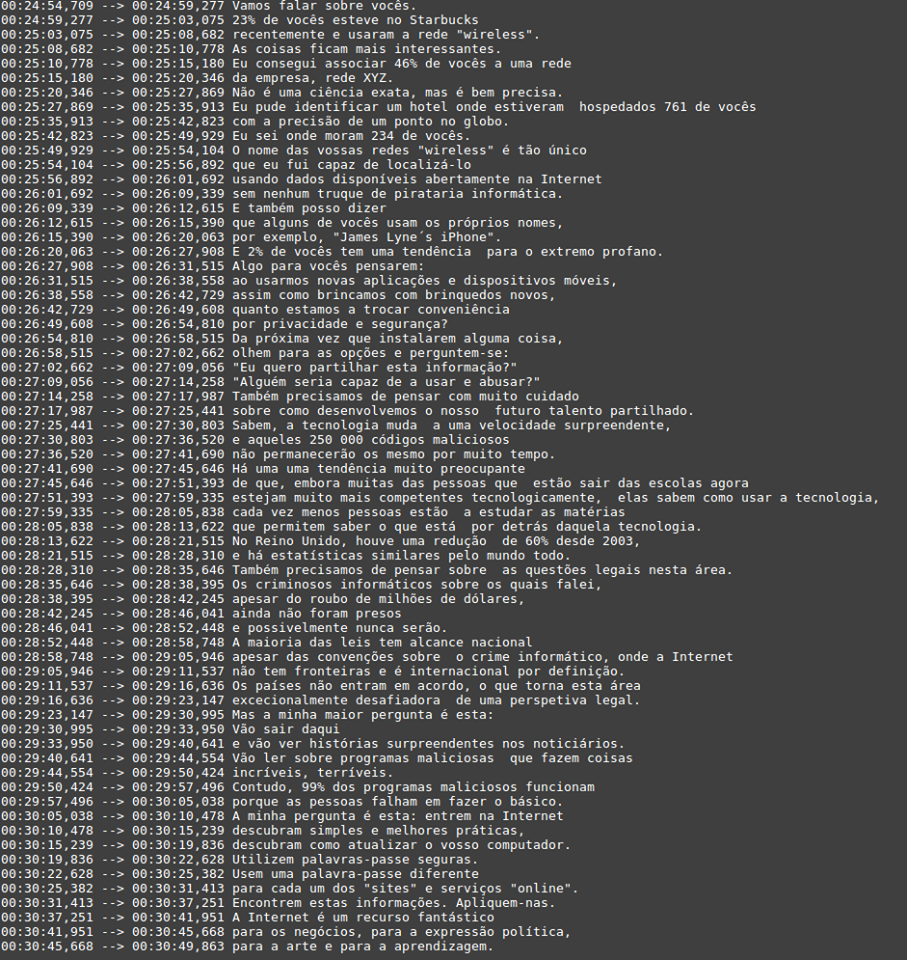
\includegraphics[scale=0.45]{7}
	\begin{figure}[!h]
	\caption{Legendas do filme Ted modificadas}
	\end{figure}
\end{center}



Como se pode observar nas legendas processadas acima, não existe qualquer tempo de silêncio presente nas legendas do filme Ted. Isto deve-se ao facto de, neste caso, quando uma legenda acaba, a seguinte aparece no ecrã, instantaneamente.
Outro facto acerca destas legendas é que o seu corpo apenas apresenta uma linha. Ou seja, não existe, no filme Ted, legendas com 2 linhas, como acontecia no caso do filme do Harry Potter.


Todas as legendas sofreram as transformações acima referidas. 
Assim sendo, o grupo concluiu o primeiro de dois exercícios do trabalho prático. 


\section{Exercício 2}
\label{sec:ex2}

O método que adotamos para resolver este problema foi o de, uma vez que as legendas têm todas um identificador que a caracteriza, alterar os timestamps consoante estes IDs.
Ou seja, se existe legendas com o mesmo identificador em ambos os ficheiros, isto quer dizer que estas legendas são iguais (apesar de estarem em linguagens diferentes).

Assim, a função que implementamos pode receber 7 argumentos : identificador da primeira legenda no ficheiro original, identificador da primeira legenda no ficheiro que vai ser consultado e alterado, identificador da última legenda no ficheiro original, identificador da última legenda a ser alterada no ficheiro, os nomes do ficheiro original, do ficheiro alterado, e por fim, do ficheiro onde tudo vai ser guardado.

\begin{center}
	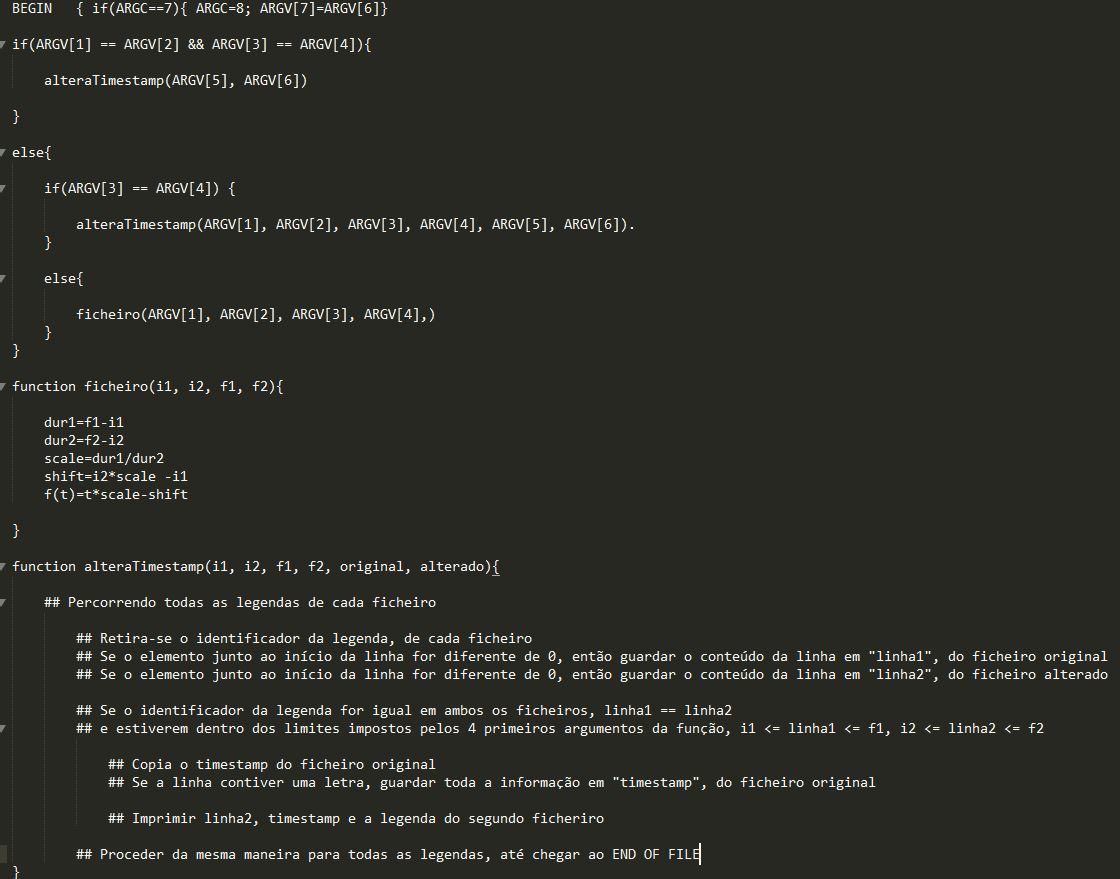
\includegraphics[scale=0.45]{9}
	\begin{figure}[!h]
	\caption{Código do exercício 2}
	\end{figure}
\end{center}
\vspace{200px}
A nossa implementação começa com uma cadeia de ifs e elses. Isto, traduzido, quer dizer que: se i1 for igual a i2, e f1 for igual a f2, então a função ficheiro não é necessária ser executada. No entanto, se a primeira condição for falsa mas f1 igual a f2, então não se deve, novamente, executar a função ficheiro, uma vez que daria um erro de divisão por 0. Por fim, se todos estas condições forem falsas, aí é executada a função ficheiro, disponibilizada pelo professor da disciplina.

Depois disto, parte-se para a função alteraTimestamp, que recebe todos os dados disponíveis como argumento.
Aqui, percorre-se as legendas dos dois ficheiros de uma forma simultânea. Assim, retira-se o identificador de ambas as legendas, e compara-se. Se estes forem iguais e estiverem dentro do limite criado pelos argumentos ([i1, f1] para a legenda do ficheiro original, [i2, f2] para a legenda do ficheiro a alterar) e copia-se o timestamp da legenda do ficheiro original.
Com todos os dados necessários, imprime-se todos eles: identificador da legenda do ficheiro alterado, novo timestamp e, também, a legenda do ficheiro alterado (o texto da legenda não sofre qualquer alteração neste processo). 

Todas as legendas percorridas, obtemos que, dentro dos limites impostos pelo utilizador, as legendas com identificadores iguais possuem o mesmo tempo de início e de fim.

Como o grupo não conseguiu implementar a 100\% as funções deste exercício, escolhemos traduzir a nossa linha de pensamento através de pseudo-código, como se pode observar na função alteraTimestamp. Deste modo, não somos capazes de fornecer um exemplo do resultado final, à semelhança de como foi feito no exercício anterior.

\vspace{500px}
\section{Conclusões}
\label{sec:conclusao}

Com este trabalho prático, adquirimos e, maioritariamente, aprofundamos os nossos conhecimentos acerca da ferramenta AWK. Com isto, constatamos toda a utilidade que esta ferramenta nos pode oferecer, sendo que agora, com estes exercícios, conseguimos dominar melhor esta linguagem de programação de processamento de texto.
Podemos afirmar que no primeiro exercício o grupo não sentiu grandes dificuldades na sua implementação, no entanto, o mesmo não se passou no exercício dois, pelas razões já referenciadas acima.
Em suma, estamos satisfeitos com o trabalho realizado até então, sendo que o grupo se sente preparado para, após este desenvolvimento dos conhecimentos em AWK que irão ser importantes no futuro, aprender e estudar uma nova ferramenta de trabalho, na qual se vai basear o próximo projeto prático.


\end{document}